\usepackage{lmodern}
\usepackage[margin=1in]{geometry}
\usepackage[dvipsnames]{xcolor}
\usepackage[a-3u,pdf17]{pdfx}
\usepackage{hyperref}
\hypersetup{colorlinks=true,linkcolor=Blue}
\usepackage[theorems,breakable]{tcolorbox}
\usepackage[shortlabels]{enumitem}
\usepackage{xfrac}
\usepackage{mathtools}
\usepackage{amssymb}
\usepackage{cleveref}
\usepackage{booktabs}
\usepackage{derivative}
\usepackage{interval}
\intervalconfig{soft open fences,separator symbol={,}}
\usepackage{graphicx}
\graphicspath{{./figures/}}
\usepackage{tikz}
\usetikzlibrary{patterns,positioning,calc}
\usepackage{pgfplots}
\pgfplotsset{samples=100} % possibly uncomment this
\pgfplotsset{compat=1.18}
\usepgfplotslibrary{fillbetween}

\definecolor{myyellow}{RGB}{255,255,168}
\definecolor{mypurple}{RGB}{216,216,255}
\definecolor{mygreen}{RGB}{216,255,216}
\definecolor{myred}{RGB}{255,216,216}
\definecolor{mycyan}{RGB}{204,229,229}

\tcbset{
    common/.style={
            fonttitle=\bfseries,
            coltitle=black,
            boxrule=0pt,
            breakable
        },
    theorem/.style={
            common,
            colback=mypurple,
            colframe=mypurple!95!black,
            fontupper=\itshape{}
        },
}

\newtcbtheorem[number within=section, crefname={definition}{definitions}]
{Definition}{DEFINITION}{
    common,
    colback=myyellow,
    colframe=myyellow!95!black
}{def}

\newtcbtheorem[use counter from=Definition, crefname={remark}{remarks}]
{Remark}{REMARK}{
    common,
    colback=mycyan,
    colframe=mycyan!95!black,
}{remark}

\newtcbtheorem[use counter from=Definition, crefname={theorem}{theorems}]
{Theorem}{THEOREM}{
    theorem
}{thm}

\newtcbtheorem[no counter]
{Proof}{Proof of}{
    common,
    colframe=black!10,
    separator sign={\!\!}
}{pf}

\newtcbtheorem[use counter from=Definition, crefname={example}{examples}]
{Example}{EXAMPLE}{
    common,
    colback=mygreen,
    colframe=mygreen!95!black,
}{ex}

\newtcbtheorem[use counter from=Definition, crefname={corollary}{corollaries}]
{Corollary}{COROLLARY}{
    theorem
}{cor}

\newtcbtheorem[use counter from=Definition, crefname={exercise}{exercises}]
{Exercise}{EXERCISE}{
    common,
    colback=myred,
    colframe=myred!95!black,
}{exercise}

\newtcbtheorem[use counter from=Definition, crefname={proposition}{propositions}]
{Proposition}{PROPOSITION}{
    theorem
}{prop}

\DeclarePairedDelimiterX\Set[1]\{\}{#1}
\DeclarePairedDelimiterX\norm[1]\lVert\rVert{#1}
\DeclarePairedDelimiterX\abs[1]\lvert\rvert{#1}
\DeclarePairedDelimiterXPP{\LN}[1]{\operatorname{\mathrm{ln}}}(){}{#1}
\DeclarePairedDelimiterXPP{\EXP}[1]{\operatorname{\mathrm{exp}}}\{\}{}{#1}

\usepackage{nicematrix}
\newcommand{\R}{\mathbb{R}}
\newcommand{\ER}{\overline{\mathbb{R}}}
\newcommand{\N}{\mathbb{N}}
\newcommand{\Z}{\mathbb{Z}}
\newcommand{\glb}{\mathrm{glb}}
\newcommand{\lub}{\mathrm{lub}}
\newcommand{\LHR}{\stackrel{\text{\tiny L'R}}{=}}
\DeclarePairedDelimiter\sequence{\langle}{\rangle}
\DeclarePairedDelimiterXPP{\bigo}[1]{\mathcal{O}}(){}{#1}

\newcommand{\Dom}{\operatorname{Dom}}
\newcommand{\Cdm}{\operatorname{Cdm}}
\title{STAT 230 - Probability}

\begin{document}

\maketitle

\tableofcontents

\newpage

\section{2020-02-03}
\underline{Roadmap}:
\begin{itemize}
    \item Review for the midterm
    \item Likelihood and the MLE for Uniform distribution
\end{itemize}
\begin{exbox}
    \begin{example}
        The average number of typos in an academic journal. A random
        sample of $ 100 $ pages are taken. Let $ y_1,\ldots ,y_{100} $
        be the observed data where $ y_i $ is the number of typos
        in page $ i $.
    \end{example}
\end{exbox}
\begin{exbox}
    \begin{example}
        Average score in STAT 231 and whether STAT 231 scores
        are correlated with STAT 230 scores.
        Let $ (x_1,y_1),\ldots ,(x_n,y_n) $ be the observed data
        where
        \begin{itemize}
            \item $ x_i= $ STAT 230 score of the $ i^{\text{th}} $ student
            \item $ y_i= $ STAT 231 score of the $ i^{\text{th}} $ student
        \end{itemize}
    \end{example}
\end{exbox}
\underline{Step 1}: Identify the population, the parameter of interest,
the type of study, variates, attributes (function of the variates), etc.

\underline{Step 2}: Collect data
\begin{itemize}
    \item Observational: None of the variables are controlled
    \item Experimental: Some variables are under the control of the person
          doing the experiment
\end{itemize}
\underline{Types of problems}
\begin{itemize}
    \item Estimation: We are trying to estimate a population attribute
    \item Hypothesis testing: Testing a claim made about the population
    \item Prediction: Predict the ``future'' value of a variate
\end{itemize}

\underline{Step 3}: Summarize data (to identify the model)
\begin{itemize}
    \item Numerical
    \item Graphical
    \item Test whether the model is appropriate
          \begin{itemize}
              \item Compare the CDF to the ECDF
              \item Compare the theoretical properties
              \item Compare the observed vs expected frequencies
          \end{itemize}
\end{itemize}

\underline{Step 4}: Do the statistical analysis based on your final model
\begin{itemize}
    \item Parameter: Unknown constant, e.g. $ \theta= $ population mean
    \item Estimate: A number that can be computed from the data set, e.g.
          $ \hat{\theta}= $ (sample mean)
    \item Estimator: The random variable from which $ \hat{\theta} $ is drawn,
          denoted $ \tilde{\theta} $.
\end{itemize}

\underline{Likelihood function}
\[ L(\theta)=\prod_{i=1}^n f(y_i;\theta) \]
where $ f= $ distribution/density function.
\[ \ell(\theta)=\ln\left[ L(\theta) \right] \]
$ \hat{\theta} $ is the MLE of $ \hat{\theta} $ that maximizes $ L(\theta) $

\underline{Measures of Association}
\begin{itemize}
    \item Data set: $ (x_1,y_1),\ldots ,(x_n,y_n) $
          \begin{itemize}
              \item $ x_i= $ number of bears you drink per week
              \item $ y_i= $ STAT 231 score in MT 1
          \end{itemize}
\end{itemize}
If $ x_i>\bar{x} $ and $ y_i<\bar{y} $, then
\[ (x_i-\bar{x})(y_i-\bar{y})<0 \]
\underline{Sample Correlation}
\[ r_{xy}=\frac{\sum\limits_{i=1}^{n} (x_i-\bar{x})(y_i-\bar{y})}{
        \sqrt{\sum\limits_{i=1}^{n} (x_i-\bar{x})^2\sum\limits_{i=1}^{n}
            (y_i-\bar{y})^2}
    }=\frac{S_{xy}}{\sqrt{S_{xx}S_{yy}}}  \]
Note that we always have $ -1\leqslant r_{xy}\leqslant 1 $.
\begin{itemize}
    \item If $ |r_{xy}|\approx 1 $, then there is evidence of a strong linear relationship
    \item If $ |r_{xy}|\approx 0 $, then there is no evidence of a linear relationship
\end{itemize}
Note that
\begin{align*}
    \sum\limits_{i=1}^{n} (x_i-\bar{x})(y_i-\bar{y})
     & =\sum\limits_{i=1}^{n} x_i y_i-n\bar{x}\bar{y} \\
     & =\sum\limits_{i=1}^{n} (x_i-\bar{x})y_i
\end{align*}
\[ \begin{array}{c|c|c}
                          & \text{Rich}              & \text{Poor}              \\
        \hline
        \text{Smoker}     & \underbrace{20}_{n_{11}} & \underbrace{80}_{n_{12}} \\
        \hline
        \text{Non-smoker} & \underbrace{50}_{n_{21}} & \underbrace{50}_{n_{22}} \\
        \hline
    \end{array} \]
\begin{align*}
    \text{Relative Risk}
     & =\frac{\frac{20}{20+80}}{\frac{50}{50+50}}                         \\
     & =\frac{\frac{n_{11}}{n_{11}+n_{12}}}{\frac{n_{21}}{n_{21}+n_{22}}}
\end{align*}

\section{2020-02-05}
\underline{Roadmap}:
\begin{itemize}
    \item Two examples
          \begin{itemize}
              \item Likelihood and the MLE for $ \uniform[0,\theta] $
              \item Discrete example
          \end{itemize}
    \item PPDAC
          \begin{itemize}
              \item Example and definitions
          \end{itemize}
\end{itemize}
\begin{exbox}
    \begin{example}\label{uniform mle}
        $ Y_1,\ldots ,Y_n $ are iid random variables with $ \uniform(0,\theta) $
        where $ \theta= $ unknown parameter (attribute) of interest.
        \begin{itemize}
            \item Data set: $ (y_1,\ldots ,y_n) $ where $ y_i>0 $ for each $ i\in[1,n] $
        \end{itemize}
        What is the MLE for $ \theta $.
        
        \textbf{Solution.}
        \[ f(y_i;\theta)=\text{density function} \]
        \[ f(y_i;\theta)=
            \begin{cases}
                \frac{1}{\theta} & 0\leqslant y_i \leqslant \theta\quad\forall i\in[1,n] \\
                0                & \text{otherwise}
            \end{cases} \]
        Therefore, the likelihood function is
        \[ L(\theta)=
            \begin{cases}
                \frac{1}{\theta^n} & 0\leqslant y_i\leqslant \theta\quad\forall i\in[1,n] \\
                0                  & \text{otherwise}
            \end{cases} \]
        Note that $ 0\leqslant y_i\leqslant \theta\quad\forall i\in[1,n]\iff
            \theta>\max\{y_1,\ldots ,y_n\} $, thus
        \[ L(\theta)=
            \begin{cases}
                \frac{1}{\theta^n} & \theta>\max \{y_1,\ldots ,y_n\} \\
                0                  & \text{otherwise}
            \end{cases} \]
        Thus, the MLE is
        \[ \hat{\theta}=\max(y_1,\ldots ,y_n) \]
    \end{example}
\end{exbox}

\begin{exbox}
    \begin{example} $ \; $
        \begin{itemize}
            \item Students come out of a classroom with equal probability
            \item There are $ N $ students in the class identified as $ \{1,\ldots ,N\} $, where
                  $ N $ is unknown
            \item We observe $ 3 $ students come out ($ 1,2,7 $)
        \end{itemize}
        What is $ \hat{N} $ given your data?
        
        \textbf{Solution.}
        \[ L(N;(1,2,7))=
            \begin{cases}
                0            & N<7          \\
                \binom{N}{3} & N\geqslant 7
            \end{cases} \]
        Given this likelihood,
        \[ \hat{N}=7 \]
        can be thought of as a discrete version of~\ref{uniform mle}.
    \end{example}
\end{exbox}

\underline{PPDAC}
A step-by-step, algorithmic approach to a statistical question.
\begin{itemize}
    \item P\@: Problem
    \item P\@: Plan
    \item D\@: Data
    \item A\@: Analysis
    \item C\@: Conclusion
\end{itemize}
\begin{exbox}
    \begin{example}
        We are interested in the attitude of Canadian residents to climate change
        (whether or not climate change is the number one issue facing the world).
        
        The area of Kitchener-Waterloo and Wellington County were selected
        and $ 200 $ people were randomly selected and interviewed.
        
        $ 126 $ of them agreed that climate change is the number one issue.
    \end{example}
\end{exbox}
\underline{Problem}
\begin{itemize}
    \item What question are we trying to answer?
    \item Types of problems:
          \begin{itemize}
              \item Descriptive: Estimating attributes of the population
              \item Causative: Check whether there is a relationship between $ x $ and $ y $
              \item Predictive: Predicting (forecasting) future values of a variate
          \end{itemize}
    \item Target population: The population of interest
          \begin{itemize}
              \item All Canadian residents
          \end{itemize}
    \item Variate: The property of the unit of the population we are interested in
          \[ y_i=
              \begin{cases}
                  0 & \text{climate change is not the number one issue} \\
                  1 & \text{otherwise}
              \end{cases} \]
    \item Attribute: A function of the variate
          \begin{itemize}
              \item $ \theta= $ proportion of Canadians who believe climate change is the number one issue
          \end{itemize}
\end{itemize}
\underline{Plan}
\begin{itemize}
    \item Study population: The population from which the sample is drawn
          \begin{itemize}
              \item The study population is \emph{usually} a subset of the target population, but
                    \textbf{does not} have to be, e.g.\ medical tests on mice.
          \end{itemize}
\end{itemize}

\section{2020-03-03}
\subsection{Accessors/Mutators (Getters/Setters), System modelling}
Advice: keep fields \code{private}

\begin{lstlisting}
    class Vec {
        int x, y;
        public:
            // accessors/getters
            int getX() const { return x; }
            int getY() const { return y; }
            // mutators/setters
            void setX(int _x) { x = _x; }
            void setY(int _y) { y = _y; }
    };
\end{lstlisting}

\subsection{I/O Operators}
\begin{itemize}
    \item standalone functions
    \item need to access fields
          \begin{itemize}
              \item Option 1: provide provide accessors/mutators
              \item Option 2: make I/O operators \code{friend}s
          \end{itemize}
\end{itemize}

\begin{lstlisting}
    class Vec {
        int x, y;
        friend ostream &operator<<(ostream &, const Vec &);
    };
\end{lstlisting}

\subsection{System Modelling}
\begin{itemize}
    \item identifying main entities (what are the main classes in the program)
    \item relationship between entities
    \item UML\@: Unified Modelling Language
\end{itemize}

A class in UML\@: (box with three sections)
\begin{enumerate}[label=(\arabic*)]
    \item Class
    \item (Optional) Fields
    \item (Optional) Methods
\end{enumerate}
An example of a class in UML is the following.
\begin{figure}[H]
    \centering
    \begin{tikzpicture}
        \umlclass{Vec}{
            - x : integer\\
            - y : integer
        }{
            + getX() : integer\\
            + setX() : integer
        }
    \end{tikzpicture}
\end{figure}
Constructors and the Big 5 are not shown.

\emph{Note}:
\begin{itemize}
    \item \code{-} \textrightarrow{} private
    \item \code{+} \textrightarrow{} public
\end{itemize}

Relationship 1: Composition (OWNS-A)
\begin{lstlisting}
    class Vec {
        int x, y;
        public:
            Vec(int, int);
            // default constructor `could' go here
    };
    class Basis {
        Vec v1, v2;
        // let's put it here instead to avoid calling Vec
        public:
            Basis() : v1{0, 1}, v2{1, 1} {}
    };
\end{lstlisting}

Basis is composed of 2 \code{Vec} objects. Instead, we write:
`Basis OWNS-A \code{Vec}.' Typically, if A OWNS-A B\@:
\begin{enumerate}[label=(\arabic*)]
    \item copying \code{A} copies \code{B} (deep)
    \item destroying \code{A} destroys \code{B}
\end{enumerate}

\begin{lstlisting}
    class List {
        Node *theList; // List OWNS-A Node
    };
\end{lstlisting}

\code{Basis} OWNS-A \code{Vec}:

\begin{figure}[H]
    \centering
    \begin{tikzpicture}
        \umlclass{Vec}{
            - x : integer\\
            - y : integer
        }{
            + getX() : integer\\
            + setX() : integer
        }
        \umlclass[x=-4,y=0]{Basis}{
            - v1 : integer\\
            - v2 : integer
        }{}
        \umlunicompo[arg=v1{,}v2,mult=2,pos=0.5]{Basis}{Vec}
    \end{tikzpicture}
\end{figure}

Relationship 2: Aggregation (HAS-A)

Typically, \code{A} HAS-A \code{B} if:
\begin{itemize}
    \item copying \code{A} does not copy \code{B} (shallow)
    \item destroying \code{A} does not destroy \code{B}
\end{itemize}

Same drawing as OWNS-A, but diamond is not shaded.

Relationship 3: Inheritance (IS-A)

\begin{figure}[H]
    \centering
    \begin{tikzpicture}
        \umlclass[x=0,y=0]{Book}{
            - title : string\\
            - author : string\\
            - numPages : integer
        }{}
        \umlclass[x=-3,y=-3]{Text}{
            - title : string\\
            - author : string\\
            - numPages : integer\\
            - topic : string
        }{}
        \umlclass[x=3,y=-3]{Comic}{
            - title : string\\
            - author : string\\
            - numPages : integer\\
            - hero: string
        }{}
        \umluniassoc{Text}{Book}
        \umluniassoc{Comic}{Book}
    \end{tikzpicture}
\end{figure}

We refer to the \code{Book} class as a:
\begin{itemize}
    \item Superclass
    \item Parent
\end{itemize}

We refer to the \code{Comic} and \code{Text} class as a:
\begin{itemize}
    \item Subclass
    \item Child
\end{itemize}

\begin{lstlisting}
    class Book {
        string title, author;
        int numPages;
        public:
            Book(string, string, int);
    };
    // public inheritance (similar to extends keyword in Java)
    class Text : public Book {
        // only need to write new field
        string topic;
        ...
    };
\end{lstlisting}

\code{Text} inherits \textbf{all} (public \textbf{and} private)
members from \code{Book}.
\begin{itemize}
    \item any method that could be called on \code{Book} can also
          be called on \code{Text}
\end{itemize}
\code{Text} has inherited the \code{private} fields.
\begin{lstlisting}
    int main() {
        Text t{...};
        t.author // cannot access this
    }
\end{lstlisting}

\begin{lstlisting}
    // will not compile (even if we changed all fields to public)
    Text::Text(string t, string a, int n, string topic) :
        title{t}, author{a}, numPages{n}, topic{topic} {}
\end{lstlisting}
\begin{itemize}
    \item Inherited fields: private in base class (\code{title}, \code{author},
          \code{numPages})
    \item MIL can only refer to fields declared by the class
\end{itemize}

\textbf{Steps of Object Construction}:
\begin{enumerate}[label=(\arabic*)]
    \item Space is allocated
    \item Superclass part is constructed
    \item Subclass' field initialization/MIL
    \item Subclass constructor runs
\end{enumerate}

\begin{lstlisting}
    Text::Text(string t, string a, int numPages, String topic) : // (1)
        Book(t, a, n), // (2) and (3)
        topic{topic} // (4)
        {}
\end{lstlisting}

Visibility: \code{protected} (UML \#)
\begin{itemize}
    \item members that are \code{protected} are visible to the class
          and its subclasses.
    \item breaks encapsulation
          \begin{itemize}
              \item child classes can break invariants
          \end{itemize}
\end{itemize}
Compromise: keep fields \code{private} but provide \code{protected}
accessors and mutators.


\section{2020-02-10}
\underline{Roadmap}:
\begin{itemize}
    \item Interval Estimation
          \subitem Likelihood Estimation
          \subitem Confidence Intervals: Coverage probabilities, Pivotal Quantities
\end{itemize}
\begin{exbox}
    \begin{example}
        The approval rating of Trump is $ 49\% $ ($ 49\% $ is the most ``likely'' value of $ \theta $)
        where $ \theta= $ population approval rating.
        \begin{itemize}
            \item What is the ``Margin of Error''?
                  \subitem How does one calculate it?
        \end{itemize}
    \end{example}
\end{exbox}
\underline{Setup} $ Y_1,\ldots ,Y_n $ are iid random variables with
distribution (density) $ f(y;\theta) $ where $ \theta= $ unknown attribute.

\underline{Objective}: Based on our data $ \{y_1,\ldots ,y_n\} $, we would
construct an interval $ [a,b] $
\[ a(y_1,\ldots ,y_n),b(y_1,\ldots ,y_n) \]
which are the ``reasonable'' values of $ \theta $.

\underline{Method 1}: Through the relative likelihood function.

\underline{Intuition}: $ \theta $ is ``reasonable'' of $ L(\theta) $
is ``close'' to $ L(\hat{\theta}) $, where $ \theta= $ MLE.

\begin{defbox}
    \begin{definition}
        A $ 100p\% $ likelihood interval for $ \theta $ where $ p\in[0,1] $
        \[ \{\theta:R(\theta)\geqslant p\} \]
    \end{definition}
\end{defbox}
Take $ p=0.5 $, we get that $ R(\theta)\geqslant 0.5 $, so
\[ \implies L(\theta)\geqslant 0.5 L(\hat{\theta}) \]
The value of the likelihood at $ \theta $ is at least $ 50\% $ of the value of the
likelihood evaluated at the MLE.

\underline{Convention}
\begin{itemize}
    \item $ R(\theta)\geqslant 0.5\implies \theta $ is very plausible
    \item $ 0.1\leqslant R(\theta)<0.5\implies \theta $ is plausible
    \item $ 0.01\leqslant R(\theta)<0.1\implies \theta $ is implausible
    \item $ R(\theta)<0.01\implies \theta $ is very implausible
\end{itemize}
\begin{exbox}
    \begin{example}
        A coin is tossed $ 200 $ times and we observe $ 120 $ heads.
        Let $ \theta=P(\text{H}) $. Is $ \theta=0.5 $ plausible?

        \textbf{Solution.} Find the $ 10\% $ likelihood interval for $ \theta $.
        \[ L(\theta)=\binom{200}{120}\theta^{120}(1-\theta)^{80} \]
        We are given that $ \hat{\theta}=0.6 $.
        \[ \left\{ \theta:\frac{\theta^{120}(1-\theta)^{80}}{0.6^{120}(0.4)^{80}}\geqslant 0.1 \right\} \]
        Thus,
        \[ R(\theta)=\frac{\theta^{120}(1-\theta)^{80}}{0.6^{120}(0.4)^{80}} \]
        Is $ \theta=0.5 $ plausible? Plug in $ \theta=0.5 $ and check if $ R(0.5)\geqslant 0.1 $.
    \end{example}
\end{exbox}
\begin{exbox}
    \begin{example}
        Two Binomial experiments.
        \begin{itemize}
            \item $ n_1=1000 $, $ y_1=200 $
            \item $ n_2=100 $, $ y_2=20 $
            \item $ y= $ number of successes
            \item $ n= $ number of trials
        \end{itemize}
        Which $ 10\% $ likelihood interval is wider?

        \textbf{Solution.} We have $ \hat{\theta}=0.2 $.
        $ n=100 $ yields a wider interval.
    \end{example}
\end{exbox}

\underline{Method 2}: Confidence intervals.

\underline{Setup}: There is a pre-specified probability (coverage probability),
say $ 95\% $ or $ 99\% $ for example.

\underline{Objective}: Based on your data, we want to estimate the (random)
interval which would contain $ \theta $ with that probability.
\begin{exbox}
    \begin{example}
        The STAT 231 scores of UW Math students is normally distributed independently
        \[ Y_i \thicksim N(\mu,64) \]
        A sample of $ 25 $ students are collected
        \[ \bar{y}=75 \]
        Find the $ 95\% $ confidence interval for $ \mu $.
    \end{example}
\end{exbox}
\underline{Sampling Distributions}

\underline{Idea}: All the data summaries are also outcomes of some random experiment.
\[ Y_1,\ldots ,Y_n \thicksim N(\mu,\sigma^2) \quad\text{iid}\]
\[ \implies \bar{Y} \thicksim N(\mu,\sigma^2/n) \]
Our sample mean $ \bar{y} $ is an outcome of this experiment.

\section{2020-03-10}
\subsection{Templates, STL, Design Patterns}
\begin{lstlisting}
    class Stack {
        int *content;
        int capacity; // capacity of array
        int length; // useful items in array
        public:
            Stack();
            void push(int);
            int top() const; // get the top of the stack
            void pop();
            ~Stack();
    };
\end{lstlisting}
Suppose we wanted a different data type from \code{int}, a \code{string}. One option
would be to manually copy the \code{.cc} and \code{.h} file and replace the types.
A better option, is to use \textbf{C++ Templates}.

\textbf{C++ template class}: a class parameterized on one or more types.
\begin{lstlisting}
    template <typename T> // T is a parameter with a type
    class Stack {
        T *content;
        int capacity; // capacity of array
        int length; // useful items in array
        public:
            Stack();
            void push(T);
            T top() const; // get the top of the stack
            void pop();
            ~Stack();
    };
\end{lstlisting}
There are only minor changes for this simple class.
\begin{lstlisting}
    stack<int> s;
    s.push(s);
    // stack where each entry of the element of the stack is another stack of type string
    stack<stack<string>> bla;
\end{lstlisting}
For the \code{List} class:
\begin{lstlisting}
    template <typename T>
    // not parameterizing the node class
    class List {
        struct Node {
            T data;
            Node *next;
        };
        ...
        public:
            class Iterator {
                Node *curr;
                Iterator(Node *);
                public:
                    T &operator*();
                    Iterator &operator++();
                    bool operator!=(Iterator &);
                    friend class List<T>;
            };
            T ith(int idx);
            void addToFront(T &);
            ~List();
    };
\end{lstlisting}
\begin{lstlisting}
    List<int> l1;
    l1.addToFront(1);
    List<List<int>> l2;
    l2.addToFront(l1);
    // a is a list of ints that are copied by value
    for(auto a : l2) { ... }
    // let's take it by reference
    for (auto &a : l2) {
        for (auto b : a) {
            cout << b;
        }
    }
\end{lstlisting}

\textbf{STL} (Standard Template Library)

\code{std::vector} are dynamic length arrays
\begin{itemize}
    \item automatically resize as needed (possibly even shrink)
\end{itemize}

\begin{lstlisting}
    // Can even be used as a Queue
    #include <vector> // ArrayList from Java
    ...
    vector<int> v; // stack allocated, empty vector
    vector<int> v{3,4}; // [3, 4]
    v.emplace_back(5); // [3, 4, 5] // automatically resizes
    // emplace_back can be more efficient than push_back as it uses move whenever
    // possible; place_back will do a copy
    v.pop_back(); // pop
    v.erase(v.begin()); // vectors have iterators
    v.erase(v.begin() + 3);
    // Suppose we wanted to traverse the vector; there are a lot of options.
    // Option 1
    for (int i = 0; i < v.size(); ++i) {
        cout << v[i]; // overloaded []
    }
    // Option 2
    for (vector<int>::iterator it = v.begin(); it != v.end(); ++it) {
        ...
    }
    // Option 3 (don't need access to the iterator)
    for (auto &i : v) {
        ...
    }
    // Option 4 (reverse iterate), no shortcut based for loop
    // r.begin() (reverse begin)
    // r.end() (reverse end)
    for (vector<int>::reverse.iterator it = v.rbegin(); it != v.rend(); ++it) {
        ...
    }
    // Option 2 and 4 can use auto in the beginning of the for loop
\end{lstlisting}

Code to an interface not to an implementation.
\begin{itemize}
    \item Create abstract classes that define the interface
    \item (Destructor needs \code{virtual} A4Q1), else memory leaks will occur
    \item Work with pointers of this abstract type
          \begin{itemize}
              \item call the interface methods
              \item use \code{virtual} methods where behaviour differs
          \end{itemize}
\end{itemize}

\subsection{Abstract Iterator Design Pattern}
\begin{lstlisting}
    class AbsIter {
        public:
            // need the virtual keyword, else breaks
            virtual int &operator*() const = 0; // pure virtual method
            virtual AbsIter &operator++() = 0;
            virtual bool operator!=(const AbsIter &) = 0;
            virtual ~AbsIter();
    };
\end{lstlisting}

\begin{lstlisting}
    class List {
        ...
        public:
            class Iterator : public AbsIter {
                ...
                public:
                    // override inherited pure virtual methods
            };
    };
\end{lstlisting}

\begin{lstlisting}
    class Set {
        public:
            class Iterator : public AbsIter {
                ...
            };
    };
\end{lstlisting}

\begin{lstlisting}
    void each(AbsIter &start, cons AbsIter &end) {
        while (start != end) {
            // do something with *start
            ++start;
        }
    }
\end{lstlisting}

\begin{lstlisting}
    template <typename Fn>
    // template function
    void foreach(AbsIter &start, const AbsIter &end, Fn f) {
        while (start != end) {
            f(*start); // can only take one parameter (possible to do more)
            ++start;
        }
    }
    void addOne(int &n) { n = n+1; }
    List l;
    // done add to front
    List::Iterator begin = l.begin();
    foreach(begin, l.end(), addOne);
\end{lstlisting}

\makeheading{2019-11-19}
Left class early due to questionable lecturer.

\makeheading{Lecture 19 | 2020-11-16}
\underline{Prediction Error}
Sometimes a key application of a fitted model
is to do \underline{prediction} on new data
(and is more important than interpretability).

Previously, we saw model selection criteria
that are computed on fitted models
(AIC, BIC, Adjusted $ R^2 $) which assess how
well the model explains the explanatory
power of a model on the \emph{data used to fit the model}
(or \emph{train}).

While these criteria incorporate penalty terms to try
to prevent overfitting, they don't directly assess
how well a model would perform in predicting the response
on new data given predictors.

We mentioned metrics such as MSPE as measures of predictive
accuracy.

To assess accuracy in prediction, we need metrics for
measuring prediction error, e.g.\ evaluated
over $ m $ observations.

\begin{itemize}
    \item Mean-squared error (MSE): If we have $ m $
          observations,
          \[ \text{MSE}=\frac{1}{m} \sum_{i=1}^{m} (y_i-\hat{y}_i)^2 \]
          where $ y_i $ is the actual value, $ \hat{y}_i $ is the
          predicted value (or equivalently, if we apply MSE on the fitted
          data, this would be the fitted value, $ \hat{\mu}_i $;
          if calculated on training data).
          Measured on the scale of $ \sigma^2 $.

          \underline{Note}: MSE is equivalently called MSPE
          if applied on new data.
    \item Root-mean-squared error (RMSE): Square root
          of MSE.\ Measured on the scale of $ \sigma $.
          \[ \text{RSME}=\sqrt{\text{MSE}} \]
    \item Mean absolute error (MAE):
          \[ \text{MAE}=\frac{1}{m} \sum_{i=1}^{m} \abs{y_i-\hat{y}_i} \]
\end{itemize}
Ideally, we have lots of data, conceptualize having three parts.
\begin{table}[ht]
    \centering
    \begin{tabularx}{\linewidth}{@{}YYY@{}}
        \toprule
        Train $ (y_1,y_2,\ldots,y_n) $ & Validation $ (y_{n+1},\ldots,y_{n+v}) $ & Test $ (y_{n+v+1},\ldots,y_{n+v+t}) $ \\
        \midrule
        \begin{itemize}
            \item $ n $ observations
            \item Fit models, as many as we want.
        \end{itemize}
                                       &
        \begin{itemize}
            \item $ v $ observations
            \item Estimate prediction error
                  for each fitted model.
        \end{itemize}
                                       &
        \begin{itemize}
            \item $ t $ observations
            \item Used at the very end for final assessment
                  of our selected model.
        \end{itemize}                                                                                        \\
        \bottomrule
    \end{tabularx}
\end{table}
We have access to train and validation. Test data is from the future,
we won't have access to this until the data is released (say
the actual stock prices were released); that is, assume we don't get
to see this.

For example, using MSE as a metric, based on a fitted model we can
compute
\begin{table}[ht]
    \centering
    \begin{tabularx}{\linewidth}{@{}YYY@{}}
        \toprule
        MSE Train & MSE Validation & MSE Test \\
        \midrule
        \[ \frac{1}{n} \sum_{i=1}^{n} (y_i-\hat{y}_i)^2 \]
                  &
        \[ \frac{1}{m} \sum_{i=n+1}^{n+v} (y_i-\hat{y_i})^2 \]
                  &
        \[ \frac{1}{t} \sum_{i=n+v+1}^{n+v+t}(y_i-\hat{y}_i)^2  \]
        \\
        \bottomrule
    \end{tabularx}
\end{table}

\begin{itemize}
    \item Observe ``MSE Train'' is equal to $ \displaystyle \frac{\SS{Res}}{n} $
          and our usual estimate of $ \hat{\sigma}^2 $
          is a scaled version of this quantity
          to compensate for the number of predictors. Specifically,
          $ \displaystyle  \hat{\sigma}^2=\frac{\SS{Res}}{n-p-1} $
          so it's unbiased.
    \item Consider ``MSE Validation'' as an \emph{estimate} of MSPE
          on new data.
    \item ``MSE Test'' is the actual test of prediction,
          we call this the \emph{actual} MSPE.\
\end{itemize}
\underline{Idea}: We hope that ``MSE Validation'' $ \approx $
``MSE Test'' since neither sets were used to fit the model.

\begin{minipage}{0.7\textwidth}
    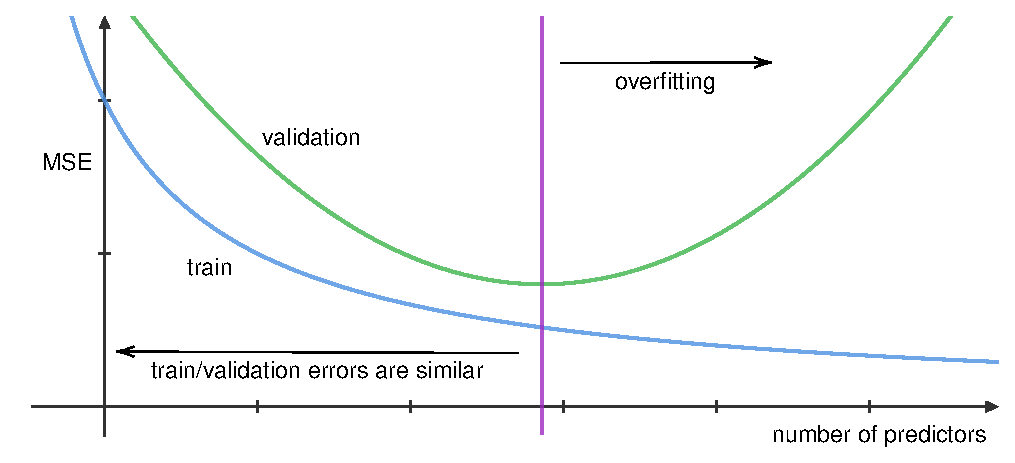
\includegraphics[width=\linewidth]{error.pdf}
\end{minipage}
\begin{minipage}{0.23\textwidth}
    \raggedright{}
    So, if we're using MSE/RMSE
    as a metric (as related to $ \hat{\sigma}^2 $ /$ \hat{\sigma} $)
    and the MSE/RMSE is significantly larger
    on validation compared to train,
    then we probably overfitted the model;
    that is, we can't expect the model
    to generalize well to new data.
\end{minipage}
\section{Cross-Validation}
How to use framework in practice:
\begin{itemize}
    \item Simplest: randomly divide available data
          between train/validation, say $ 80\% $/$ 20\% $ split.

          Weakness:
          \begin{enumerate}
              \item Don't use all data for training.
              \item Only get one estimate of prediction error.
          \end{enumerate}
    \item Better: Use cross-validation scheme (CV). How to
          do CV with $ K $ folds:
          \begin{figure}[!ht]
              \centering
              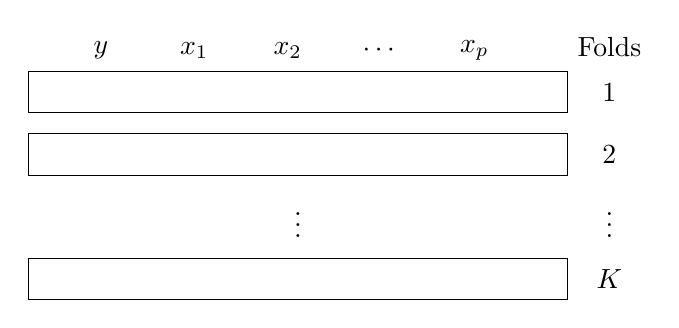
\begin{tikzpicture}[x=0.75pt,y=0.75pt,yscale=-1,xscale=1]
                  \draw (10,30) -- (270,30) -- (270,50) -- (10,50) -- cycle ;
                  \draw (10,60) -- (270,60) -- (270,80) -- (10,80) -- cycle ;
                  \draw (10,120) -- (270,120) -- (270,140) -- (10,140) -- cycle ;
                  \draw (140,100) node {$\vdots $};
                  \draw (290,40) node {$1$};
                  \draw (290,70) node {$2$};
                  \draw (290,100) node {$\vdots $};
                  \draw (290,130) node {$K$};

                  \draw (45,20) node {$y$};
                  \draw (90,20) node {$x_{1}$};
                  \draw (135,20) node {$x_{2}$};
                  \draw (180,20) node {$\cdots $};
                  \draw (225,20) node {$x_{p}$};
                  \draw (290,18) node {Folds};
              \end{tikzpicture}
          \end{figure}
          \begin{itemize}
              \item Divide available data for train and validation
                    into $ K $ roughly equally sized sets (folds),
                    usually randomly.
              \item For CV $ k $, use data in fold $ k $
                    as validation, and train on
                    the rest of data.
              \item Thus, to estimate the prediction error
                    \emph{for a given model}, we fit it $ K $ times, each
                    time treating the data in folds, $ 1,2,\ldots,K $
                    as validation.
                    Therefore, we get $ K $ estimates of prediction error
                    for that particular model.
              \item For example, using RMSE, we get
                    \[ \overline{\text{RSME}}
                        =\text{RMSE}_1,\text{RMSE}_2,\ldots,\text{RSME}_K \]
                    and can take the average
                    \[ \frac{1}{K} \sum_{k=1}^{K}\text{RSME}_k \]
                    as an estimate for RMSPE on new data (test set).
          \end{itemize}
\end{itemize}

\makeheading{Lecture 20 | 2020-11-18}
\section{Combining Cross Validation With Model Selection}
\begin{itemize}
      \item Given some candidate models (e.g., with different
            variables included) we can do $ K $-fold
            cross-validation using each of them, and choose the one
            with the lowest average prediction error across
            the folds, e.g., $ \displaystyle
                  \frac{1}{K} \sum_{k=1}^{K} \text{RSME}_k $.
      \item How to choose $ K $? Some common choices are:
            \begin{itemize}
                  \item $ K=5 $
                  \item $ K=10 $
                  \item $ K=N $ (number of observations for train/valid).
                        This is commonly known as ``leave one out'' (LOO).
            \end{itemize}
            The more folds, the higher the computational time, but
            it can give a better estimate of prediction error.
      \item What if we are not given a list of models to compare?
            (and if there are too many predictors to do all possible
            regressions). Then, we can combine cross-validation with
            \emph{model selection procedures} (criteria based on training
            data and search strategy).
\end{itemize}
To estimate the prediction error for a given
\emph{model selection procedure} we apply it $ K $ times,
each time treating observations in fold $ 1,2,\ldots,K $
as validation sample, e.g., use the \emph{average}
RMSE and choose the model selection procedure
with the lowest estimated prediction error.

\underline{Note}: actual variables selected in each fold might
be different.

\underline{Recommendation}: apply chosen
model selection \emph{procedure} (lowest estimated prediction error)
to the entire set of observations available for training
and validation to get a final model (for applications
to test data).

Recall we have:
\begin{itemize}
      \item $ \text{AIC}=2q-2\ln[L(\hat{\theta})] $
      \item $ \text{BIC}=q\ln(n)-2\ln[L(\hat{\theta})] $
\end{itemize}
We can go further (and beyond \emph{PLUS ULTRA!}) and consider the following.
\begin{Definition}{$ L_0 $ Penalized Likelihood}{}
      For any $ \lambda>0 $,
      \[ q\lambda -2\ln[L(\hat{\theta})] \]
\end{Definition}
\underline{Beyond Stepwise Regression}
\begin{itemize}
      \item Stepwise is a deterministic algorithm which is fast,
            but might not give optimal model selected.
      \item Could try stochastic algorithm, e.g., iterative
            conditional minimization (ICM)
\end{itemize}

\section{Iterative Conditional Minimization}
Start with a model with just intercept.
For a given random seed, take predictors $ x_1,\ldots,x_p $
and randomly re-order them into $ x_{(1)},\ldots,x_{(p)} $.
For $ j=1,\ldots,p $: (let $ \mathcal{S} $ be the predictors
currently in model, so start at $ \mathcal{S}=\emptyset $).
\begin{itemize}
      \item If $ x_{(j)} $ is not in $ \mathcal{S} $:
            \begin{itemize}
                  \item Fit model with $ \mathcal{S} $.
                        If addition of $ x_{(j)} $ improves criterion,
                        then add $ x_{(j)} $ to $ \mathcal{S} $.
            \end{itemize}
      \item If $ x_{(j)} $ is in $ \mathcal{S} $:
            \begin{itemize}
                  \item Fit model removing $ x_{(j)} $. If excluding
                        $ x_{(j)} $ improves criterion, then remove
                        $ x_{(j)} $ from $ \mathcal{S} $.
            \end{itemize}
\end{itemize}
Repeat for loop until no predictors are added/removed
from an entire pass through the for loop.
\begin{Remark}{}{}
      Different random orderings could give different
      sets $ \mathcal{S} $ at end of procedure, could pick one
      that has the best criterion overall.
\end{Remark}

\section{Lecture 21}
A \emph{continuous random variable} $ X $ maps points in a continuous
sample space to real numbers such that the range is uncountably infinite.

\textsc{Examples of continuous random variables}

Let $ X $ be the number the point spots at.
\begin{enumerate}[(1)]
    \item temperature of a day
    \item length of time until a bus arrives
    \item height of a random person
    \item by (3)/\# of people (avg height of 3)
\end{enumerate}

$F(x)=P(X\le x)$, $F(a)=P(X\le a) $

\subsection{Example}
For $ x<0 $, no chance of the point stopping at a number $ <0 $.

For $ x>4 $, $ F(x)=1 $ since the point is certain to stop at a number
below $ 4 $.

$ P(0<x\le 1)=\frac{1}{4}=F(1) $

\[ F(x)=\begin{cases}
    0,\, x<0\\
    \frac{x}{4},\,0\le x\le 4 \\
    1,\,x>4
\end{cases} \]

\textsc{Properties of $ F(x) $}

(1) For all $ x $, $ P(X=x)=0 $. So,
\begin{align*}
    P(a<x\le b)&=P(a\le x\le b)\\
    &=P(a<x<b)\\
    &=P(a\le x<b)
\end{align*}
\begin{remark}
    End points don't matter.
\end{remark}

(2) \begin{align*}
    \lim\limits_{{\epsilon} \to {0}} F(x)-F(x-\epsilon)&=
    \lim\limits_{{\epsilon} \to {0}} P(x-\epsilon<X\le x)\\
    &=P(X=x)\\
    &=0
\end{align*}
Thus $ \lim\limits_{{\epsilon} \to {0}} F(x-\epsilon)=F(x) $, so
$ F(x) $ is continuous.

(3) $ F(x) $ is non-decreasing.

(4) $ \lim\limits_{{x} \to {+\infty}} F(x)=1 $,
$ \lim\limits_{{x} \to {-\infty}} F(x)=0 $

(5) $ 0\le F(x)\le 1 $

\begin{defbox}
    \subsubsection{Definition (Probability Density Function)}
    The \emph{probability density function} (p.d.f) $ f(x) $ for a continuous
    random variable $ X $ is the derivative
    \[ f(x)=\frac{d}{dx}F(x) \]
    where $ F(x) $ is the cumulative distribution function for $ X $.
\end{defbox}

\begin{remark}
    $ f(x) $ is not a probability. It can be $ >1 $ relative
    likelihood that $ X $ takes a value near $ X $.
\end{remark}

\textsc{Properties of $ f(x) $}

(1)
\begin{align*}
    P(a\le X\le b)&=F(b)-F(a)\\
    &=\int\limits_{a}^{b} f(x) d{x}
\end{align*}

(2)
\begin{align*}
    \int\limits_{-\infty}^{+\infty} f(x) d{x}&=F(+\infty)-F(-\infty)\\
    &=1-0\\
    &=1
\end{align*}

(3) $ f(x)\ge 0 $ (since $ F(x) $ is non-decreasing, it's derivative is non-negative)

(4) \[ F(x)=\int\limits_{-\infty}^{x} f(u) d{u} \]

\subsection{Example}
Suppose a continuous random variable $ X $ is on the range $ [0,1] $ has the 
cumulative distribution function $ F(x)=x^2 $.

\textsc{What is the probability density function?}

$ f(x)=\frac{d}{dx} F(x)=2x $.

\textsc{What is $ P(X=0.25) $?}

$ P(X=0.25)=0 $

\textsc{What is $ P(X\le 0.25) $?}

(1) $ P(X\le 0.25)=F(0.25)=(0.25)^2=0.0625 $

(2)
\[  P(X\le 0.25)=
\int\limits_{0}^{0.25} f(x) d{x} =\int\limits_{0}^{0.25} 2x d{x} =0.625 \]

\begin{defbox}
    Expectation:
    \[ E[X]=\int\limits_{-\infty}^{+\infty} xf(x) d{x} =
    \int\limits_{x\in\text{range}}^{} xf(x) d{x}  \]
\end{defbox}

\begin{defbox}
    Variance:
    \[ Var(X)=E[X^2]-E[X]^2=\int\limits_{-\infty}^{+\infty} x^2f(x) d{x}-
    \int\limits_{-\infty}^{+\infty} xf(x) d{x} \]
\end{defbox}

\begin{defbox}
    \subsubsection{Definition (Percentiles)}
    The $ p^\text{th} $ \emph{percentile} of a distribution $ x_p $ such that
    $ F(x_p)=p $.
\end{defbox}
\makeheading{Lecture 22 | 2020-11-22}
\begin{Example}{}{}
    $ X_1,\ldots,X_n $ are i.i.d.\
    \begin{enumerate}
        \item $ \exponential{\theta} $
        \item $ \uniform{0,\theta} $
        \item $ f(x;\theta)=\theta x^{\theta-1} $ with $ 0<x<1 $ and $ \theta>0 $
    \end{enumerate}
    \textbf{Solution.}
    \begin{enumerate}
        \item $ \exponential{\theta} $. $ \mu_1=\E{X_1}=\theta $. $ \mu_1(\theta)=\theta $
              \[ \hat{\mu}_1=\frac{1}{n} \sum_{i=1}^{n} X_i \]
              $ \mu_1(\hat{\theta})=\hat{\mu}_1 $. Since $ \mu_1 $ is the identity
              map,
              \[ \hat{\theta}=\hat{\mu}_1=\frac{1}{n} \sum_{i=1}^{n} X_i \]
        \item $ \uniform{0,\theta} $.
              \[ \mu_1=\E{X_1}=\int_{0}^{\theta} x\biggl(\frac{1}{\theta} \biggr)\, d{x}=
                  \theta/2 \]
              $ \mu_1(\theta)=\frac{\theta}{2} $
              \[ \hat{\mu}_1=\frac{1}{n} \sum_{i=1}^{n} X_i \]
              \[ \mu_1(\hat{\theta})=\frac{\hat{\theta}}{2} =\hat{\mu}_1 \]
              Therefore,
              \[ \hat{\theta}_{\text{MM}}=2\hat{\mu}_1=\frac{2}{n} \sum_{i=1}^{n} X_i \]
        \item $ f(x;\theta)=\theta x^{\theta-1} $ with $ 0<x<1 $ and $ \theta>0 $
              \[ \mu_1=\E{X_1}=\int_{0}^{1} x \theta x^{\theta-1}\, d{x}=
                  \frac{\theta}{1+\theta} \]
              $ \displaystyle \mu_1(\theta)=\frac{\theta}{1+\theta} $
              \[ \hat{\mu}_1=\frac{1}{n}\sum_{i=1}^{n}  X_i \]
              \[ \mu_1(\hat{\theta})=\frac{\hat{\theta}}{1+\hat{\theta}}=\hat{\mu}_1 \]
              Therefore,
              \[ \hat{\theta}_{\text{MM}}=\frac{\hat{\mu}_1}{1-\hat{\mu}_1}=\frac{\bar{X}}{1-\bar{X}}   \]
        \item $ X_1,\ldots,X_n\stackrel{\text{iid}}{\sim}\N{\mu,\sigma^2} $.
              \[ \theta=\begin{pmatrix}
                      \mu \\
                      \sigma^2
                  \end{pmatrix} \]
              \begin{align*}
                  \mu_1 & =\E{X_1}=\mu                                  \\
                  \mu_2 & =\E{X_1^2}=\Var{X}+[\E{X_1}]^2=\mu^2+\sigma^2
              \end{align*}
              \begin{align*}
                  \mu_1(\mu,\sigma^2) & =\mu            \\
                  \mu_2(\mu,\sigma^2) & =\mu^2+\sigma^2
              \end{align*}
              \[ \hat{\mu}_1=\frac{1}{n} \sum_{i=1}^n X_i \]
              \[ \hat{\mu}_2=\frac{1}{n} \sum_{i=1}^{n} X_i^2 \]
              \[ \mu_1(\hat{\mu},\hat{\sigma}^2)=\hat{\mu}=\hat{\mu}_1=\bar{X} \]
              \[ \mu_2(\hat{\mu},\hat{\sigma}^2)=(\hat{\mu})^2+\hat{\sigma}^2=\hat{\mu}_2 \]
              Therefore,
              \begin{align*}
                  \hat{\mu}_{\text{MM}} & =\bar{X}_n                                    \\
                  \hat{\sigma}^2_{\text{MM}}
                                        & =\hat{\mu}_2-(\bar{X}_n)^2                    \\
                                        & =\frac{1}{n} \sum_{i=1}^{n} X_i^2-\bar{X}_n   \\
                                        & =\frac{1}{n} \sum_{i=1}^{n} (X_i-\bar{X}_n)^2
              \end{align*}
    \end{enumerate}
\end{Example}
\section{Maximum Likelihood Method}
This section: introduce the most commonly used method for estimating unknown
parameter $ \theta $ referred to as maximum likelihood method.
\begin{itemize}
    \item Likelihood function
          \begin{enumerate}
              \item Suppose $ X_1,\ldots,X_n $ are i.i.d.\ from $ f(x;\theta) $
              \item Given $ (x_1,\ldots,x_n) $, the observed value of $ (X_1,\ldots,X_n) $.
                    We calculate the joint p.f.\ of $ (X_1,\ldots,X_n) $ at observed
                    data $ (x_1,\ldots,x_n) $ or joint p.d.f.\ of $ (X_1,\ldots,X_n) $
                    at observed data $ (x_1,\ldots,x_n) $.

                    Discrete random variables joint p.d.f.\ of $ (X_1,\ldots,X_n) $
                    at $ (x_1,\ldots,x_n) $:
                    \[ \Prob{X_1=x_1,\ldots,X_n=x_n}=
                        \prod_{i=1}^n \Prob{X_i=x_i}=
                        \prod_{i=1}^n f(x_i;\theta) \]
                    Continuous random variables joint p.d.f.\ of $ (X_1,\ldots,X_n) $
                    at $ (x_1,\ldots,x_n) $:
                    \[ f_{X_1,\ldots,X_n}(x_1,\ldots,x_n)=
                        \prod_{i=1}^n f(x_i;\theta) \]
              \item We use $ L(\theta;x_1,\ldots,x_n) $ or simply
                    $ L(\theta) $ to denote it. That is to say,
                    \[ L(\theta;x_1,\ldots,x_n)=
                        \begin{cases*}
                            \Prob{X_1=x_1,\ldots,X_n=x_n} & discrete\\
                            f_{X_1,\ldots,X_n}(x_1,\ldots,x_n) & continuous
                        \end{cases*}=\prod_{i=1}^n f(x_i;\theta) \]
                    Here, $ L(\theta;x_1,\ldots,x_n) $ is called the likelihood function
                    of $ \theta $.
          \end{enumerate}
\end{itemize}
Comments:
\begin{enumerate}
    \item Likelihood function measures how likely we get
          the observed data for a given $ \theta $.
    \item Smaller $ L(\theta) $ means $ \theta $ is less likely
          to generate the observed data.
    \item Larger $ L(\theta) $ means $ \theta $ is more likely
          to generate the observed data.
\end{enumerate}
\underline{Idea of Maximum Likelihood Method}

Choose $ \theta $ to maximize $ L(\theta) $ or choose
$ \theta $ such that it most likely generates the observed data.

Maximum likelihood estimator/estimate (MLE)
\begin{enumerate}
    \item ML estimate maximizes $ L(\theta) $ and we use
          $ \hat{\theta}=\hat{\theta}(x_1,\ldots,x_n) $ to denote it.
          \[ \hat{\theta}=\hat{\theta}(x_1,\ldots,x_n)=
              \arg\max_{\theta\in \Theta}L(\theta) \]
    \item ML estimator: $ \hat{\theta}=\hat{\theta}(X_1,\ldots,X_n) $
    \item Log-likelihood function: log of likelihood function:
          \[ \ell(\theta)=\ln[L(\theta)] \]
          Then: an immediate result is:
          \[ \hat{\theta}=\hat{\theta}(x_1,\ldots,x_n)=
              \arg\max_{\theta\in \Theta}\ell(\theta)
              \arg\max_{\theta\in \Theta}L(\theta) \]
    \item Invariance principal of ML estimator
          $ \tau(\theta) $ is a function of $ \theta $.
          $ \tau(\hat{\theta}) $ is the ML estimator of
          $ \tau(\theta) $ if $ \hat{\theta} $ is the ML
          estimator of $ \theta $.
\end{enumerate}
\begin{Example}{}{}
    $ X_1,\ldots,X_n \stackrel{\text{iid}}{\sim} \poi{\theta} $.
    Find ML estimator of $ \theta $.

    \textbf{Solution.}
    \[ f(x;\theta)=\frac{\theta^x}{x!} e^{-\theta} \]
    \[ L(\theta)=\prod_{i=1}^n f(x_i;\theta)=
        \prod_{i=1}^n \frac{\theta^{x_i}}{x_i!}e^{-\theta}=
        \frac{\theta^{\sum_{i=1}^{n} x_i}}{\prod_{i=1}^n(x_i!)}e^{-n\theta}   \]
    \[ \ell(\theta)=\biggl(\sum_{i=1}^{n} x_i\biggr)\ln(\theta)-n \theta-
        \sum_{i=1}^{n} \ln(x_i!) \]
    \[ \frac{d\ell(\theta)}{d\theta}=\frac{\sum_{i=1}^{n} x_i}{\theta}-n   \]
    ML estimator of $ \theta $ satisfies
    \[ \biggl[\frac{d\ell}{d\theta}\biggr]_{\theta=\hat{\theta}}=0\implies
        \frac{\sum_{i=1}^{n} x_i}{\hat{\theta}}-n=0\implies
        \hat{\theta}=\frac{\sum_{i=1}^{n} x_i}{n}   \]
    ML estimator of $ \theta $ is
    \[ \hat{\theta}=\frac{\sum_{i=1}^{n} X_i}{n}\quad\text{(same as the MM estimator)} \]
\end{Example}
\begin{Remark}{}{}
    \begin{itemize}
        \item ML estimator of $ \theta^2 $ is $ (\hat{\theta})^2 $
        \item ML estimator of $ e^{-\theta} $ is $ e^{-\hat{\theta}} $
    \end{itemize}
\end{Remark}
\begin{Example}{}{}
    $ X_1,\ldots,X_n $ are i.i.d.\ from $ f(x;\theta)=\theta x^{\theta-1} $
    with $ 0<x<1 $, $ \theta>0 $.
    Find ML estimator of $ \theta $.

    \textbf{Solution.}
    \[ L(\theta)=\prod_{i=1}^n f(x_i;\theta)=
        \prod_{i=1}^n \theta x_i^{\theta-1}=\theta^n\biggl(\prod_{i=1}^n x_i \biggr)^{\theta-1} \]
    \[ \ell(\theta)=n\ln(\theta)+(\theta-1)\sum_{i=1}^{n} \ln(x_i) \]
    \[ \frac{d\ell(\theta)}{d\theta}=\frac{n}{\theta} +\sum_{i=1}^{n} \ln(x_i)  \]
    ML estimate $ \hat{\theta} $ satisfies
    \[ \biggl[\frac{d\ell}{d\theta}\biggr]_{\theta=\hat{\theta}}=0\implies
        \frac{n}{\hat{\theta}} +\sum_{i=1}^{n} \ln(x_i)=0
        \implies \hat{\theta}=-\frac{n}{\sum_{i=1}^{n} \ln(x_i)}  \]
    ML estimator:
    \[ \hat{\theta}=-\frac{n}{\sum_{i=1}^{n} \ln(X_i)}\quad\text{(is different from MM estimator)} \]
\end{Example}

\makeheading{Lecture 23 | 2020-11-29}
\begin{Example}{}{}
    Suppose $ X_1,\ldots,X_n\stackrel{\text{iid}}{\sim}\N{\mu,\sigma^2} $.
    Find ML estimator of $ \theta $.

    \textbf{Solution.}
    \[ L(\mu,\sigma^2)=\prod_{i=1}^n f(x_i;\mu,\sigma^2) \]
    \begin{align*}
        \ell(\mu,\sigma^2)
         & =\sum_{i=1}^{n}\ln[f(x_i;\mu,\sigma^2)]                  \\
         & =\sum_{i=1}^{n} \ln\biggl[\frac{1}{\sqrt{2\pi \sigma^2}}
        \expon*{-\frac{(x_i-\mu)^2}{2\sigma^2}} \biggr]             \\
         & =\sum_{i=1}^{n}
        \biggl[-\frac{(x_i-\mu)^2}{2\sigma^2}-
            \frac{1}{2} \ln(2\pi\sigma^2) \biggr]
    \end{align*}
    \[ \frac{\partial\ell}{\partial\mu}=
        \frac{\sum_{i=1}^{n} (\mu-x_i)}{\sigma^2}   \]
    \[ \frac{\partial\ell}{\partial \sigma^2}=
        \frac{\sum_{i=1}^{n} (x_i-\mu)^2}{2\sigma^4}-
        \biggl(\frac{n}{2}\biggr)\biggl(\frac{1}{\sigma^2} \biggr)   \]
    ML estimate satisfies
    \begin{align*}
        \frac{\sum_{i=1}^{n} (X_i-\hat{\mu})^2}{\hat{\sigma}^2}    & =0 \\
        \frac{\sum_{i=1}^{n} (X_i-\hat{\mu})}{2(\hat{\sigma}^2)^2}-
        \biggl(\frac{n}{2}\biggr)\biggl(\frac{1}{\sigma^2} \biggr) & =0
    \end{align*}
    \begin{align*}
        \hat{\mu}      & =\frac{1}{n} \sum_{i=1}^{n} X_i               \\
        \hat{\sigma}^2 & =\frac{1}{n} \sum_{i=1}^{n} (X_i-\hat{\mu})^2
    \end{align*}
    ML estimator of $ (\mu,\sigma^2) $ is
    \begin{align*}
        \hat{\mu}    & =\frac{1}{n} \sum_{i=1}^{n}X_i=\bar{X}_n     \\
        \hat{\sigma} & =\frac{1}{n}\sum_{i=1}^{n} (X_i-\bar{X}_n)^2
    \end{align*}
    which is the same as MM estimator.
\end{Example}
\begin{Example}{}{}
    \[ f(x,\theta)=\begin{dcases}
            \frac{1}{\theta} & 0\le x\le \theta \\
            0                & \text{otherwise}
        \end{dcases} \]
    Note that the support of $ X $ depends on $ \theta $.
    Find ML estimator of $ \theta $.

    \textbf{Solution.}
    \[ L(\theta)=\prod_{i=1}^n f(x_i;\theta)
        =\begin{dcases}
            \biggl(\frac{1}{\theta} \biggr)^{\!n} & 0\le x_1,\ldots,x_n\le \theta \\
            0                                     & \text{otherwise}
        \end{dcases}=
        \begin{dcases}
            \frac{1}{\theta^n} & 0\le x_{(1)},x_{(n)}\le \theta \\
            0                  & \text{otherwise}
        \end{dcases} \]
    \begin{itemize}
        \item $ \theta<x_{(n)} $, $ L(\theta)=0 $
        \item $ \theta\ge x_{(n)} $, $ L(\theta) $
              is a strictly monotone decreasing function of $ \theta $.
    \end{itemize}
    This implies that the ML estimate of $ \theta $
    is
    \[ x_{(n)}=\max(x_1,\ldots,x_n) \]
    ML estimator of $ \theta $ is
    \[ \hat{\theta}=\max_{1\le i\le n}X_i=X_{(n)} \]
    is different from the MM estimator $ \hat{\theta}_{\text{MM}}=2\bar{X}_n $.

    Which estimator is better? $ \hat{\theta}_{\text{MM}} $
    or $ \hat{\theta}_{\text{ML}} $? STAT 450 covers this.
    \begin{itemize}
        \item Biased or unbiased estimator. Let $ \hat{\theta} $
              denote one estimator of $ \theta $. If $ \E{\hat{\theta}}=\theta $,
              then $ \hat{\theta} $ is an unbiased estimator of $ \theta $.
              Otherwise, $ \hat{\theta} $ is a biased estimator of $ \theta $.
    \end{itemize}
\end{Example}
\section{Properties of ML Estimator}
In this section:
\begin{enumerate}
    \item We only consider the case that the support of $ X_1,\ldots,X_n $
          does not depend on $ \theta $.
    \item We talk about random variables, only concerned
          about ML estimator.
    \item We only consider $ \theta $ is 1-dimensional or $ \theta $
          is a scalar.
\end{enumerate}
We define some notation first.
\begin{Definition}{Score Function}{}
    The \textbf{score function} is defined as
    \[ S(\theta)=S(\theta;\symbf{x})=
        \frac{d}{d\theta}\ell(\theta)=
        \frac{d}{d\theta}\ln[L(\theta)]   \]
    where $ \symbf{x} $ are the observed data.
    When the support of $ X_1,\ldots,X_n $ does not depend
    on $ \theta $, then $ S(\hat{\theta})=0 $.
\end{Definition}
\begin{Definition}{Information Function}{}
    The \textbf{information function} is defined as
    \[ I(\theta)=I(\theta;\symbf{x})=-\frac{d^2}{d\theta^2}\ell(\theta)=
        -\frac{d^2}{d\theta^2}\ln[L(\theta)]   \]
    where $ \symbf{x} $ are the observed data. $ I(\hat{\theta}) $
    is called the \textbf{observed information}.
\end{Definition}
\begin{Definition}{Fisher Information/Expected Information}{}
    The \textbf{fisher information} (\textbf{expected information})
    is defined as
    \[ J(\theta)=\E{I(\theta;\symbf{X})}=-\E*{\frac{d^2}{d\theta^2}\ell(\theta;
            \symbf{X}) } \]
    where $ \symbf{X} $ is the potential data.

    In particular, when $ \symbf{X}=(X_1,\ldots,X_n) $
    is i.i.d.\ from $ f(x,\theta) $, then
    \[ \ell(\theta;\symbf{x})=\sum_{i=1}^{n} \ln[f(x_i;\theta)] \]
    \[ I(\theta;\symbf{X})=-\frac{d^2
        }{d\theta^2} \sum_{i=1}^{n}\ln[f(X_i;\theta)]
        =-\sum_{i=1}^{n} \frac{d^2}{d\theta^2}\ln[f(X_i;\theta)]   \]
    Therefore,
    \[ J(\theta)=\E*{-\sum_{i=1}^{n} \frac{d^2}{d\theta^2}\ln[f(X_i;\theta)]}
        =-\E*{\frac{d^2}{d\theta^2}\ln[f(X_1;\theta)]} \]
\end{Definition}
\begin{Definition}{Fisher Information of One Observation}{}
    The \textbf{fisher information of one observation}
    is
    \[ J_1(\theta)=-n\E*{\frac{d^2}{d\theta^2}\ln[f(X_1;\theta)]}  \]
    The \textbf{fisher information in $ \symbf{n} $ observations} is
    \[ J(\theta)=n J_1(\theta) \]
\end{Definition}
\begin{Example}{}{}
    Suppose $ X_1,\ldots,X_n\stackrel{\text{iid}}{\sim}\poi{\theta} $.

    \[ L(\theta;\symbf{x})=\prod_{i=1}^n f(x_i;\theta) \]
    \[ \ell(\theta;\symbf{x})=\sum_{i=1}^{n}
        \ln[f(x_i;\theta)]=\sum_{i=1}^{n}
        \ln\biggl[\frac{\theta^{x_i}e^{-\theta}}{x!} \biggr]=
        \biggl(\,\sum_{i=1}^{n} x_i\biggr)\ln(\theta)-
        n\ln(\theta)-\sum_{i=1}^{n} \ln(x_i!) \]
    Score function:
    \[ S(\theta;\symbf{x})=\frac{\partial}{\partial\theta}\ell(\theta;\symbf{x})
        =\frac{\sum_{i=1}^{n} x_i}{\theta}-n   \]
    Observed information function:
    \[ I(\theta;\symbf{x})=
        -\frac{\partial S}{\partial \theta}S(\theta;\symbf{x})
        =\frac{\sum_{i=1}^{n} x_i}{\theta^2}   \]
    Fisher information:
    \[ J(\theta)=\E{I(\theta;\symbf{X})}=
        \E*{\frac{\sum_{i=1}^{n} X_i}{\theta^2}}=
        \frac{n\E{X_1}}{\theta^2}=\frac{n\theta}{\theta^2}=\frac{n}{\theta}  \]
    Recall that: $ \displaystyle \hat{\theta}_{\text{ML}}=\frac{\sum_{i=1}^{n} X_i}{n} $
    \[ \implies \Var{\hat{\theta}_{\text{ML}}}=
        \frac{\Var{X_i}}{n}=\frac{\theta}{n}  \]
    Is there any relationship between $ J(\theta) $
    and $ \Var{\hat{\theta}_{\text{ML}}} $?
\end{Example}
\begin{Theorem}{Cramér–Rao Bound}{}
    The variance of any unbiased estimator
    $ \hat{\theta} $ of $ \theta $ is bounded by the reciprocal
    of the Fisher information $ J(\theta) $:
    \[ \Var{\theta}\ge \frac{1}{J(\theta)}  \]
\end{Theorem}
\begin{Corollary}{}{}
    If $ T $ is an unbiased estimator of $ g(\theta) $, then
    \[ \Var{T}\ge \frac{[g^\prime(\theta)]^2}{J(\theta)} \]
\end{Corollary}
\begin{Theorem}{}{}
    ML estimator satisfies (when support of $ X_1,\ldots,X_n $
    does not depend on $ \theta $)
    \begin{enumerate}[label=(\arabic*)]
        \item $ \hat{\theta}\stackrel{\mathbb{P}}{\to}\theta $
              as $ n\to\infty $.
        \item $ \displaystyle \sqrt{n}(\hat{\theta}-\theta)\stackrel{\text{d}}{\to}
                  \N*{0,\frac{1}{J_1(\theta)}} $
        \item By delta-method,
              $ \displaystyle \sqrt{n}(g(\hat{\theta})-g(\theta))\stackrel{\text{d}}{\to}
                  \N*{0,\frac{[g^\prime(\theta)]^2}{J_1(\theta)} } $
    \end{enumerate}
\end{Theorem}
\begin{Remark}{}{}
    (1) Tells us that $ \hat{\theta} $ is close to $ \theta $
    as $ n\to\infty $.

    (2) Tells us that $ \displaystyle \sqrt{n}(\hat{\theta}-\theta)\approx
        \N*{0,\frac{1}{J_1(\theta)}}\implies
        \hat{\theta}\approx \N*{\theta,\frac{1}{nJ_1(\theta)}}=\N*{
            \theta,\frac{1}{J(\theta)}
        } $
    \[ \Var{\hat{\theta}}\approx \frac{1}{J(\theta)}  \]
    which is the CR lower-bound. $ \E{\hat{\theta}}\approx \theta $.
    \begin{itemize}
        \item $ \hat{\theta} $ is asymptotically unbiased.
        \item $ \hat{\theta} $ is asymptotically efficient.
    \end{itemize}

    (3) Tells us that $ \displaystyle  g(\hat{\theta})\approx \N*{g(\theta),
            \frac{[g^\prime(\theta)]^2}{J(\theta)}} $.
    \begin{itemize}
        \item $ g(\hat{\theta}) $ is asymptotically unbiased.
        \item $ \displaystyle \Var{g(\hat{\theta})}\approx
                  \frac{[g^\prime(\theta)]^2}{J(\theta)} $
              which is the CR lower-bound.
    \end{itemize}
\end{Remark}
Conclusion: ML estimator is asymptotically optimal.

\makeheading{2020-03-06}
\section{Burst Error Correcting}
``Cyclic codes are good for (cyclic) burst error correcting.''

Suppose we have a $ C:(n,k,d) $ code, with $ e=\lfloor \frac{d-1}{2} \rfloor=5 $.
In practice, errors typically happen in bursts (not spread out).
We expect typically one burst per codeword, or bursts to carry through
two codewords.

\begin{defbox}
    \begin{definition}
        Let $ \bm{e}\in V_n(F) $. The \textbf{cyclic burst length of $\bm{e}$}
        is the length of the smallest cyclic block that contain all the non-zero
        entries of $ \bm{e} $.
    \end{definition}
\end{defbox}

\begin{exbox}
    \begin{example}
        $ \bm{e}=\bm{011}00000\bm{1} $ has cyclic burst length $ 4 $.
    \end{example}
\end{exbox}

\begin{defbox}
    \begin{definition}
        We say $ \bm{e} $ is a \textbf{cyclic burst error of length $ \bm{t} $} if its cyclic
        burst length is $ t $.
    \end{definition}
\end{defbox}

\begin{defbox}
    \begin{definition}
        A linear code $ C $ is a \textbf{$ \bm{t} $-cyclic burst error correcting code}
        if every cyclic burst error of length at most $ t $ lies in a unique coset
        of $ C $. The largest such $ t $ is called the \textbf{cyclic burst error capability
            of $ \bm{C} $}.
    \end{definition}
\end{defbox}

\begin{exbox}
    \begin{example}
        $ g(x)=1+x+x^2+x^3+x^6 $ generates a $ (15,9) $-binary cyclic code $ C $
        that is a $ 3 $-cyclic burst error correcting code.
    \end{example}
\end{exbox}

$ d(C)\leqslant 5 $, so $ e\leqslant 2 $. We verify this by checking that
each cyclic burst of length $ \leqslant 3 $ has a unique syndrome.

\begin{table}[H]
    \centering
    \begin{tabularx}{\linewidth}{@{}YYY@{}}
        Cyclic burst errors & Syndromes  & Notes                                   \\
        \midrule
        \midrule
        0                   & 000000                                               \\
        \midrule
        $ x^0 $             & 100000                                               \\
        $ x^1 $             & 010000                                               \\
        $ x^2 $             & 001000                                               \\
        $ x^3 $             & 000100                                               \\
        $ x^4 $             & 000010                                               \\
        $ x^5 $             & 000001                                               \\
        $ x^6 $             & 111100     & $ x^6+g(x)\iff (0000001)+(1111001) $    \\
        $ x^7 $             & 011110                                               \\
        $ x^8 $             & 001111                                               \\
        $ x^9 $             & 111011     & $ x^9+g(x)\iff (0001111)+(1111001) $    \\
        $ x^{10} $          & 100001     & $ x^{10}+g(x)\iff (0111011)+(1111001) $ \\
        $ x^{11} $          & 101100     & $ x^{11}+g(x)\iff (0100001)+(1111001) $ \\
        $ x^{12} $          & 010110                                               \\
        $ x^{13} $          & 001011                                               \\
        $ x^{14} $          & 111001     & $ x^{14}+g(x)\iff (0001011)+(1111001) $ \\
        \midrule
        $ 1+x $             & 110000                                               \\
        $ x(1+x) $          & 011000                                               \\
        $ \vdots $          & $ \vdots $                                           \\
        $ x^{14}(1+x) $     & 011001                                               \\
        \midrule
        $ 1+x+x^2 $         & 111000                                               \\
        $ x(1+x+x^2) $      & 011100                                               \\
        $ \vdots $          & $ \vdots $                                           \\
        $ x^{14}(1+x+x^2) $ & 001001                                               \\
        \midrule
        $ 1+x^2 $           & 101000                                               \\
        $ x(1+x^2) $        & 010100                                               \\
        $ \vdots $          & $ \vdots $                                           \\
        $ x^{14}(1+x^2) $   & 101001                                               \\
    \end{tabularx}
\end{table}
The number of cyclic bursts of length $ \leqslant 3 $ is $ 61 $.
The number of syndromes is $ 64 $.

\begin{exbox}
    \begin{example}
        $ g(x)=1+x^4+x^6+x^7+x^8 $ generates a $ (15,7) $-binary cyclic
        code that is $ 4 $-cyclic burst error correcting.
        Distance $ \leqslant 5 $ so $ e\leqslant 2 $.
    \end{example}
\end{exbox}

\textbf{Question}: How to construct codes with high cyclic burst error
correcting capability?
\begin{enumerate}[label=(\arabic*)]
    \item Use a computer search
    \item RS Codes
    \item Interleaving
\end{enumerate}

\begin{thmbox}
    \begin{theorem}
        Let $ C $ be an $ (n,k,d) $-code over $ GF(q) $. Let $ t $ be its
        cyclic burst error correcting capability.
        \[ \left\lfloor \frac{d-1}{2} \right\rfloor \leqslant t \leqslant n-k \]
    \end{theorem}
\end{thmbox}

\begin{proof}
    Every cyclic burst of length $ \leqslant t $ has weight $ \leqslant t $.
    Since every vector of weight $ \leqslant \lfloor \frac{d-1}{2} \rfloor $
    has a unique syndrome, we have $ \lfloor \frac{d-1}{2} \rfloor \leqslant t $.

    The number of cyclic burst errors where all the non-zero entries lie in the first
    $ t $ coordinate positions is $ q^t $. Each of them has a unique coset
    and the total number of cosets is $ q^{n-k} $. Thus,
    \[ q^t\leqslant q^{n-k}\implies t\leqslant n-k \]
\end{proof}

Exercise: Prove that $ t\leqslant \frac{n-k}{2} $.

\section{Decoding Cyclic Burst Errors}
Let $ C $ be a $ t $-cyclic burst error correcting code generated
by $ g(x) $ which is a degree-$ k $ monic divisor of $ x^n-1 $ over $ GF(q) $.

Recall: A PCM for $ C $ is:
\[ H= \Bigl[\; I_{n-k}\mid -R^\top \;\Bigr] \]

whose columns are $ x^0 \mod g(x),\ldots ,x^{n-1} \mod g(x) $.

The syndrome of $ r(x) $ is $ s(x)\equiv r(x)\mod g(x) $.

\textbf{Idea:} Suppose $ \bm{e} $ is a cyclic burst of length $ \leqslant t $.

Compute $ \bm{s}=H\bm{r}^\top\equiv r(x)\mod g(x) $.

Suppose $ \bm{e}= $ \fbox{x o $ \cdots $ o x x x} . We multiply $ x^3 $ by $ \bm{e} $,
so we get \fbox{x x x x o $ \cdots $ o}.

$ \bm{s}=H\bm{r}^\top=H\bm{e}^\top $.

$ \bm{s}_1=H(x\bm{r})^\top = H(x\bm{e})^\top $

$ \bm{s}_2=H(x^2\bm{r})^\top = H(x^2\bm{e})^\top $

$ \bm{s}_3=H(x^3\bm{r})^\top = H(x^3\bm{e})^\top $

\section{Lecture 25.00: F Test}
\begin{figure}[!htbp]
    \centering
    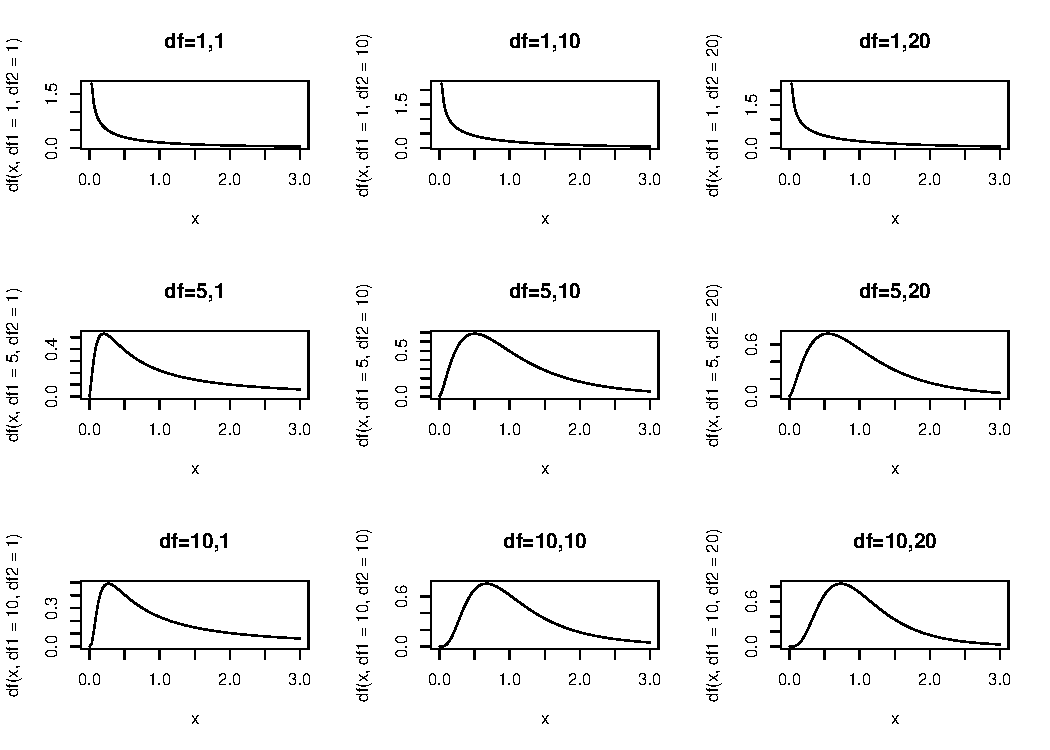
\includegraphics[width=0.7\textwidth]{fdistn.pdf}
    \caption{$ F $ distribution}
\end{figure}
\begin{Theorem}{}{}
    Let $ X \sim \chi^2(m) $ and $ Y \sim \chi^2(n) $, then
    \[ \frac{X/m}{Y/n} \sim F(m,n) \]
\end{Theorem}
\begin{Theorem}{}{}
    Let $ X \sim F(m,n) $ and $ Y \sim 1/X $, then
    \[ Y \sim F(n,m) \]
\end{Theorem}
\begin{Example}{}{}
    $ \alpha=\Prob{F(20,4)>4}=(0.05,0.1) $ since
    \begin{center}
        \begin{NiceTabular}{c|ccc}
            $\alpha$       & 0.1  & 0.05 & 0.01 \\
            \midrule
            critical value & 3.84 & 5.80 & 14.0
        \end{NiceTabular}
    \end{center}
    In R, we can directly calculate $ \alpha $ with \code{1-pf(4,20,4)=0.094}.
\end{Example}
\[ \tilde{F}=\frac{\widetilde{\MS{Trt}}}{\widetilde{\MS{Res}}}  \]
Now, $ \widetilde{\MS{Res}}=\tilde{\sigma}^2 $. We know
\begin{equation}\label{eq:1}
    \frac{\tilde{\sigma}^2\text{df}_\text{Res}}{\sigma^2} \sim \chi^2(\text{df}_{\text{Res}})
\end{equation}
Similarly,
\begin{equation}\label{eq:2}
    \frac{\widetilde{\MS{Trt}}\text{df}_\text{Trt}}{\sigma^2} \sim \chi^2(\text{df}_\text{Trt})
\end{equation}
Divide~\ref{eq:2} by~\ref{eq:1} to get
\[ \frac{\widetilde{\MS{Trt}}}{\widetilde{\MS{Res}}} \sim F(n,d) \]
where $ n=\text{df}_\text{Trt} $ and $ d=\text{df}_\text{Res} $.

\subsection*{When is $ F $ large?}
\[ \E{\tilde{F}}=
    \E*{\frac{\widetilde{\MS{Trt}}}{\widetilde{\MS{Res}}}}{\color{red}\approx}
    \frac{\E{\widetilde{\MS{Trt}}}}{\E{\widetilde{\MS{Res}}}}
    =\frac{\sigma^2+r \dfrac{\sum_{i=1}^t \tau_i^2}{t-1} }{\sigma^2}  \]
\[ \E{\tilde{F}}=1+\frac{r}{\sigma^2} \frac{\sum_{i=1}^t \tau_i^2 }{t-1}  \]
If $ \tau_1=\tau_2=\cdots=\tau_t=0 $, then $ \E{\tilde{F}}=1 $.
However, if even one $ \tau $ is not zero, then $ \E{\tilde{F}}>1 $.

\subsection*{$F$ Test}
\begin{enumerate}[(1)]
    \item $ H_0 $: $ \tau_1=\tau_2=\cdots=\tau_t=0 $ versus $ H_a $: at least one $\tau$ is not zero.
    \item $ \displaystyle d=\frac{\MS{Trt}}{\MS{Res}}  $ where $ D \sim F(\text{df}_\text{Trt},\text{df}_\text{Res}) $
    \item $ p\text{-value}=\Prob{D>d} $
    \item Conclusion.
\end{enumerate}

\section{Lecture 26}
\textbf{Example}

If $ Z \thicksim N(0,1) $, find $ d $ such that $ P(|Z|<d)=0.9 $.
\begin{align*}
    P(|Z|<d)&=P(-d<Z<d)\\
    &=P(Z<d)-P(Z>-d)\\
    &=P(Z\le d)-\left[ 1-P(Z\le d) \right]\\
    &=2P(Z\le d)-1
\end{align*}
\begin{align*}
    &2P(Z\le d)-1=0.90\\
    &\implies P(Z\le d)=\frac{0.90+1}{2}\\
    &\implies F(d)=0.95\\
    &\implies F^{-1}(F(d))=F^{-1}(0.95)\\
    &\implies d=1.6449
\end{align*}

\subsection{Basic Terminology and Techniques (9.1)}
We have models for a single RV (both discrete or cont.) but we often
care about two or more RV's at the same time (and their relationship)
Examples:
\begin{itemize}
    \item two stock returns
    \item heights and weights
    \item number of cards of a rank vs number of a suit
    \item treatment vs recovery time
    \item all machine learning classification and regression
\end{itemize}
In this course, we focus on all discrete random variables

\begin{defbox}
    \subsection{Definition (Joint Probability Function)}
    Let $ X_1,\ldots,X_n $ be $ n $ discrete random variables.
    We define the \emph{joint probability function} $ f(x_1,\ldots,x_n) $ of
    $ (X_1,\ldots,X_n) $ as
    \begin{align*}
        f(x_1,\ldots,x_n)&=P(X_1=x_1 \text{ and } \cdots \text{ and } X_n=x_n)\\
        &=P(X_1=x_1,\ldots,X_n=x_n)
    \end{align*}
\end{defbox}

\begin{thmbox}
    \subsection{Theorem}
    \begin{itemize}
        \item $ \sum\limits_{\text{all } (x_1,\ldots,x_n)} f(x_1,\ldots,x_n)=1 $
        \item $ f(x_1,\ldots ,x_n)\ge 0 $ for all $ (x_1,\ldots,x_n) $
    \end{itemize}
\end{thmbox}

\textbf{Example}

Suppose we flip a coin 3 times. Let $ X= $ \# heads.
Let
\[ Y=\begin{cases}
    1,\,\text{ if first flip is a H}\\
    0,\, \text{ otherwise}
\end{cases} \]
Find $ f(x,y) $.

\begin{tabular}{| *{5}{>{\centering\arraybackslash}p{2cm} |}}
    \hline
    $y\backslash x$ & 0 & 1 & 2 & 3\\
    \hline
    $0$ & $ \nicefrac{1}{8}$ & $ \nicefrac{2}{8} $ & $ \nicefrac{1}{8} $ & $\nicefrac{0}{8} $\\
    \hline
    $1$ & $ \nicefrac{0}{8}$ & $ \nicefrac{1}{8} $ & $ \nicefrac{2}{8} $ & $\nicefrac{1}{8} $\\
    \hline
\end{tabular}
$ f(x,y) $ can be represented in a table or as a function of $ x $ and $ y $
(not usually a histogram).

Now suppose we are only interested in one of the random variables. e.g. suppose
we are only want to find out about $ X $.
\[ P(X=x)=f(0,0)+f(0,1)=\frac{1}{8} +0=\frac{1}{8} \]

\begin{defbox}
    \subsection{Definition (Marginal Probability Function)}
    Let $ X $ and $ Y $ be two discrete random variables.
    We define the \emph{marginal probability function} of $ X $ as
    \[ f_X(x)=\sum\limits_{\text{all } y}f(x,y) \]
    and the \emph{marginal probability function} of $ Y $ as
    \[ f_Y(y)=\sum\limits_{\text{all } x}f(x,y) \]
\end{defbox}

\begin{defbox}
    \subsection{Definition (Independent Random Variables)}
    $ X_1,\ldots,X_n $ are \emph{independent random variables} if
    and only if
    \[ f(x_1,\ldots ,x_n)=f_1(x_1)\cdots f_n(x_n) \]
    for all $ (x_1,\ldots,x_n) $.
\end{defbox}
From example: Are $ X $ and $ Y $ independent? No.
$ f(0,0)=\frac{1}{8} \neq f_X(0)f_Y(0)=\frac{1}{8}\cdot \frac{1}{2} $
Shortcut: any $ 0 $ in your table $ \rightarrow $ dependent.

\section{2020-03-13}
\underline{Roadmap}:
\begin{enumerate}[label=(\roman*)]
    \item Recap and the relationship between Confidence and Hypothesis
    \item Example: Bias Testing
    \item Testing for variance (Normal)
    \item What if we don't know how to construct a Test-Statistic?
\end{enumerate}

\begin{exbox}
    \begin{example}
        $ Y_1,\ldots Y_n $ iid $ N(\mu,\sigma^2) $
        \begin{itemize}
            \item $ \sigma^2= $ known
            \item $ \mu= $ unknown
            \item Sample: $ \{y_1,\ldots ,y_n\} $
            \item $ \bar{y}= $ sample mean
            \item $ H_0 $: $ \mu=\mu_0 $ where $ \mu_0 $ is given
            \item $ H_1 $: $ \mu \neq \mu_0 $
        \end{itemize}
        \[
            \begin{aligned}
                D= & \left|\frac{\bar{Y}-\mu_0}{\frac{\sigma}{\sqrt{n}}} \right|
                   & \quad                                                       & \rightarrow &  & \text{Test-Statistic (r.v.)}       \\
                d= & \left|\frac{\bar{y}-\mu_0}{\frac{\sigma}{\sqrt{n}}} \right|
                   &                                                             & \rightarrow &  & \text{Value of the Test-Statistic}
            \end{aligned}
        \]
        \[
            \begin{aligned}
                p\text{-value}
                 & =P(D\geqslant d)   & \quad & \text{assuming }H_0\text{ is true} \\
                 & =P(|Z|\geqslant d) &       & Z \sim N(0,1)
            \end{aligned}
        \]
    \end{example}
\end{exbox}
\underline{Question}: Suppose the $ p $-value for the test $ >0.05 $
if and only if $ \mu_0 $ belongs in the $ 95\% $ confidence interval for $ \mu $?

YES\@.

Suppose $ \mu_0 $ is in the $ 95\% $ confidence interval for $ \mu $, i.e.
\[ \bar{y}\pm 1.96 \frac{\sigma}{\sqrt{n}} \]
\[ \begin{aligned}
        \mu_0\leqslant \bar{y}+1.96 \frac{\sigma}{\sqrt{n}} \\
        \mu_0\geqslant \bar{y}-1.96 \frac{\sigma}{\sqrt{n}}
    \end{aligned}
\]
These two equations yield
\[ d=\left|\frac{\bar{y}-\mu_0}{\frac{\sigma}{\sqrt{n}}} \right|\leqslant 1.96 \]
\[ p\text{-value}=P(|Z|\geqslant d)>0.05 \]

\underline{General result} (assuming same pivot)

$ p $-value of a test $ H_0 $: $ \theta=\theta_0 $ vs $ H_1 $: $ \theta\neq \theta_0 $
is more than $ q\% $, then $ \theta_0 $ belongs to the $ 100(1-q)\% $
confidence interval and vice versa.

\begin{exbox}
    \begin{example}[Bias]
        A $ 10 $ kg weight is weighed $ 20 $ times ($ y_1,\ldots ,y_n $).
        \begin{itemize}
            \item $ \bar{y}=10.5 $
            \item $ s=0.4 $
            \item $ H_0 $: The scale is unbiased
            \item $ H_1 $: The scale is biased
        \end{itemize}
        If the scale was unbiased,
        \[ Y_1,\ldots ,Y_n \sim N(10,\sigma^2) \]
        If the scale was biased,
        \[ Y_1,\ldots ,Y_n \sim N(10+\delta,\sigma^2) \]
        \begin{itemize}
            \item $ H_0 $: $ \delta=0 $ (unbiased)
            \item $ H_1 $: $ \delta\neq 0 $ (biased)
        \end{itemize}
        is equivalent to
        \begin{itemize}
            \item $ H_0 $: $ \mu=10 $
            \item $ H_1 $: $ \mu\neq 10 $
        \end{itemize}
        Test-statistic:
        \[ D=\left|\frac{\bar{Y}-10}{\frac{S}{\sqrt{n}}} \right| \]
        Compute $ d $.
        \[ d=
            \left|\frac{\bar{y}-10}{\frac{s}{\sqrt{n}}} \right|=
            \left|\frac{10.5-10}{\frac{0.4}{\sqrt{20}}} \right|=5.59017 \]
        \[
            \begin{aligned}
                p\text{-value}
                 & =P(D\geqslant d)                             \\
                 & =P(|T_{19}|\geqslant 5.59)                   \\
                 & = 1-P(|T_{19}|\leqslant 5.59)                \\
                 & =1-\left[ 2P(T_{19}\leqslant 5.59)-1 \right] \\
                 & \approx 1-(2-1)                              \\
                 & =0
            \end{aligned}
        \]
        Very strong evidence against $ H_0 $.
    \end{example}
\end{exbox}

\begin{exbox}
    \begin{example}[Draw Conclusions]
        $ Y_1,\ldots ,Y_n = $ co-op salaries. $ Y_1,\ldots ,Y_n \sim N(\mu,\sigma^2) $
        \begin{itemize}
            \item $ H_0 $: $ \mu=3000 $
            \item $ H_1 $: $ \mu<3000 $ ($ \mu\neq 3000 $)
        \end{itemize}
        \[ D=\left|\frac{\bar{Y}-\mu_0}{\frac{S}{\sqrt{n}}} \right| \]
        \[ D=
            \begin{cases}
                0                                        & \bar{Y}>\mu_0 \\
                \frac{\bar{Y}-\mu_0}{\frac{S}{\sqrt{n}}} & \bar{Y}<\mu_0
            \end{cases} \]
    \end{example}
\end{exbox}
If $ n $ is large, then
\[ Y_1,\ldots ,Y_n \sim f(y_i;\theta) \]
\begin{itemize}
    \item $ H_0 $: $ \theta=\theta_0 $
    \item $ H_1 $: $ \theta\neq \theta_0 $
\end{itemize}
\[ \Lambda(\theta)=-2\ln\left[ \frac{L(\theta_0)}{L(\tilde{\theta})} \right] \]
where $ \Lambda $ satisfies all the properties of $ D $. Also,
\[ \lambda(\theta)=-2\ln\left[ \frac{L(\theta_0)}{L(\hat{\theta})}\right]
    =-2\ln\left[ R(\theta_0) \right] \]
and
\[ p\text{-value}=P(\Lambda\geqslant \lambda)=P(Z^2\geqslant \lambda) \]

\section{Lecture 28.00: Model 7}
\begin{Definition}{Randomized block design, Model 7}{}
    The \textbf{randomized block design} (RBD) is defined as
    \[ Y_{ij}=\mu+\tau_i+\beta_j+R_{ij}\quad(R_{ij} \sim \N{0,\sigma^2}) \]
    where $ \beta_j $ is the $ j^{\text{th}} $ block (BIK) effect. Note that
    \begin{itemize}
        \item $ i=1,2,\ldots,t $
        \item $ j=1,2,\ldots,r $
        \item $ \sum_{i=1}^t \tau_i=0  $
        \item $\sum_{j=1}^{r} \beta_j=0$
    \end{itemize}
\end{Definition}
\begin{Example}{LS for Model 7}{}
    The LS for Model 7 is
    \[ W=\sum_{ij}r_{ij}+\lambda_1\biggl(\sum_{i=1}^{t} \tau_i\biggr)+
        \lambda_2 \biggl(\sum_{j=1}^{r} \beta_j\biggr)  \]
    Solving
    \[ \hat{\mu}=\bar{y}_{++} \]
    \[ \hat{\tau}_i=\bar{y}_{i+}-\bar{y}_{++} \]
    \[ \hat{\beta}_j=\bar{y}_{+j}-\bar{y}_{++} \]
    \[ \hat{\sigma}^2=\frac{W}{(rt)-(t+r+1)+2} \]
\end{Example}


\end{document}